\section{Ciclo de vida de software}

Engenheiros de software tem tradicionalmente considerado qualquer trabalho após
o primeiro lançamento de um software simplesmente como manutenção. Alguns
pesquisadores no entanto tem dividido este trabalho em atividades distintas, incluindo
adaptação, prevenção, correção, entre outras, mas sempre considerando manutenção
basicamente uniforme ao longo do tempo \cite{rajlich2000staged}.

Entretanto, estudos recentes tem demonstrado que esta visão, onde manutenção
ocupa um papel basicamente uniforme ao longo do tempo, não explica muito bem o
desenvolvimento de software na maior parte dos cenários, e uma das abordagens
para explicar o fenômeno tem colocado a atividade de manutenção distribuída ao
longo do ciclo de vida do software \cite{rajlich2000staged}.

\subsection{Staged Model for Software Evolution}

O modelo {\it Staged Model for Software Evolution} \cite{rajlich2000staged},
proposto como forma de interpretar os estágios de evolução do ciclo de vida de um software,
possui cinco estágios distintos de evolução,
conforme ilustrado na Figura \ref{staged-model-cycle}. Neste modelo, cada
estágio possui atividades distintas, necessidades e
ferramentas variadas, e consequencias diversas em relação ao negócio.

\begin{description}
  \item [{\it Initial development.}]
    Engenheiros desenvolvem a primeira versão funcional do sistema.
  \item [{\it Evolution.}]
    Engenheiros expandem as capacidades e funcionalidades do sistema para
    atender as necessidades dos usuários.
  \item [{\it Servicing.}]
    Engenheiros fazem pequenos reparos em defeitos e mudanças funcionais
    simples.
  \item [{\it Phaseout.}]
    A empresa decide não mais oferecer serviços com o software, procurando
    gerar receita com o sistema pelo maior tempo possível.
  \item [{\it Closedown.}]
    A empresa retira o sistema do mercado e direciona os usuários para um novo
    sistema, se houver.
\end{description}

%Our work has been influenced by Franz Lehner, 2
%who provided empirical evidence that activities and
%their frequency change during a system’s life cycle.
%Manny Lehman 3 documented the inevitability of the
%evolution stage, demonstrating increases in size, com-
%plexity, and functionality during evolution.

As atividades realizadas em cada atividade variam em relação ao tipo e
frequência, na fase Evolution, por exemplo, ocorre inclusão de novas
funcionalidades, em Servicing a maior parte das alterações em código são
correções, apresentando pouca atividade com grandes mudanças mas com mudanças
frequentes enquanto durar este ciclo.

\begin{figure}[h]
  \center
  \includegraphics[scale=0.6]{imagens/staged-model-cycle.png}
  \caption{O modelo de evolução {\it staged model} consiste em cinco etapas \cite{rajlich2000staged}.}
  \label{staged-model-cycle}
\end{figure}

O retorno de uma fase para outra anterior pode representar um alto custo e alto
risco, devendo ser realizado com cautela e conhecimento deste fato. Os
usuários devem saber em que estágio um software está antes de adquirir um
produto de software, estamos falando de produtos de software comerciais
tradicionais, para o qual este modelo de evolução foi designado e proposto.

%Transitions from one stage to the next can result
%from deliberate business decisions or by default or
%mistake. Managers must be conscious of the enormous
%business consequences of unintentional transitions and
%be aware of their symptoms so they can halt or reverse
%them while there is still time. Managers should also
%understand that attempts to return to previous stages
%or to deal with software as if it’s in a previous stage can
%be both expensive and risky.

%Customers should know what stage software is in
%and should explicitly ask for that information before
%buying it. They should avoid any software in the
%advanced servicing stage because the software is
%unlikely to evolve with the user’s needs, and close-
%down is probably near.

%• Each stage has very different technical solutions,
%processes, staff needs, and management activi-
%ties.
%• Managers who have a better understanding of
%stage transitions, their characteristics, and infor-
%mation flow across them can plan better.
%• Keeping systems within a particular stage for as
%long as possible is important.
%• Developers must design systems to allow high
%flexibility during evolution because managers can-
%not predict what new user requirements will arise.

O software acadêmico, no entando, aproxima-se muito mais de um modelo de
software livre do que de software comercial tradicional, uma vez que usualmente
não possuem empresas comercializando o software acadêmico, além de estar
frequentemente disponível em repositórios de código fonte, e em
alguns casos, ser distribuído usando licenças de software livre.

\subsection{Ciclo de vida de software acadêmico}

Este modelo de evolução do software em estágios, no entanto, foi avaliado e adaptado
ao contexto de software livre \cite{capiluppi2007adapting}, e diante as
semelhanças com o software acadêmico, este modelo adaptado ao software livre serve ao propósito de ser
utilizado para
avaliar a evolução do software acadêmico, a Figura \ref{staged-model-foss-cycle}
apresenta o modelo de evolução adaptado ao software livre, adotado
neste estudo como aplicável também ao software acadêmico.

\begin{figure}[h]
  \center
  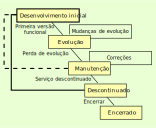
\includegraphics[scale=0.6]{imagens/staged-model-foss-cycle.png}
  \caption{O modelo de evolução {\it staged model} adaptado a software livre \cite{capiluppi2007adapting}.}
  \label{staged-model-foss-cycle}
\end{figure}

A primeira diferença observada é em relação a fase Initial development,
dependendo da definição de ``fase inicial'' muitos projetos de software livre
podem nunca ter saído desta fase, assim é também para o software acadêmico. Em respeito aos lançamentos,
em sistemas comerciais tradicionais eles devem ser completos, rodando e autorizado
pela empresa detentora, enquanto no mundo do software livre é comum
permitir acesso público ao código em repositórios de código fonte, seguindo
um modelo de ``versão permanente''.

A segunda diferença é relacionada a possibilidade de laços entre
as fases Evolution e Servicing. Muitos projetos de software livre
possuem fases de congelamento na adição de novas funcionalidades ({\it freeze})
enquanto permanece numa fase de Servicing até o descongelamento, voltando
a Evolution.

A terceira diferença está na comunidade de software livre,
novos times de desenvolvimento são formados ao longo do tempo
com a saída de desenvolvedores antigos e a entrada de novos.
E projetos em fase Phaseout podem experimentar um renascimento
retornando ao período de Evolution.

Apesar das diferenças, o autor \citeonline{capiluppi2007adapting} demonstram em experimentos e
revisão de literatura que o modelo adaptado pode ser utilizado para
compreender evolução de software livre, e diante as similaridades entre software livre
e software acadêmico, este modelo poderá, consequentemente, ser também
utilizado para compreender a evolução e ciclo de vida do software acadêmico.
